% This is a template file for Sweave used in MAGeCK
% Author: Wei Li, Shirley Liu lab
% Do not modify lines beginning with "#__".
\documentclass{article}

\usepackage{amsmath}
\usepackage{amscd}
\usepackage[tableposition=top]{caption}
\usepackage{ifthen}
\usepackage{fullpage}
\usepackage[utf8]{inputenc}
% \usepackage{longtable}

\usepackage{Sweave}
\begin{document}
\Sconcordance{concordance:all_countsummary.tex:all_countsummary.Rnw:1 13 1 1 0 14 1 1 %
141 5 1 1 16 23 0 1 2 1 8 23 0 1 2 4 1 1 8 23 0 1 2 23 1 2 2 3 1 2 2 6 %
1 4 2 5 1 2 2 8 1}

\setkeys{Gin}{width=0.9\textwidth}

\title{MAGeCK Count Report}
\author{Wei Li}

\maketitle


\tableofcontents

\section{Summary}

%Function definition

%__FILE_SUMMARY__

The statistics of comparisons are listed in Table 1 and Table 2.
The corresponding fastq files in each row are listed in Table 3.

% latex table generated in R 4.4.1 by xtable 1.8-4 package
% Fri Aug 16 17:18:01 2024
\begin{table}[ht]
\centering
\begin{tabular}{ccccc}
  \hline
 & Label & Reads & Mapped & Percentage \\ 
  \hline
1 & Low\_1 & 43718952 & 43718952 & 1.00 \\ 
  2 & Low\_1 & 45560656 & 45560656 & 1.00 \\ 
  3 & Low\_2 & 40553489 & 40553489 & 1.00 \\ 
  4 & Low\_2 & 42377934 & 42377934 & 1.00 \\ 
  5 & Low\_3 & 51495403 & 51495403 & 1.00 \\ 
  6 & Low\_3 & 54023585 & 54023585 & 1.00 \\ 
  7 & High\_1 & 37337429 & 37337429 & 1.00 \\ 
  8 & High\_1 & 38986079 & 38986079 & 1.00 \\ 
  9 & High\_2 & 37941677 & 37941677 & 1.00 \\ 
  10 & High\_2 & 39892307 & 39892307 & 1.00 \\ 
  11 & High\_3 & 44368672 & 44368672 & 1.00 \\ 
  12 & High\_3 & 46403720 & 46403720 & 1.00 \\ 
   \hline
\end{tabular}
\caption{Summary of comparisons} 
\label{tab:one}
\end{table}
% latex table generated in R 4.4.1 by xtable 1.8-4 package
% Fri Aug 16 17:18:01 2024
\begin{table}[ht]
\centering
\begin{tabular}{ccccc}
  \hline
 & Label & TotalsgRNA & ZeroCounts & GiniIndex \\ 
  \hline
1 & Low\_1 & 21339 & 660 & 0.10 \\ 
  2 & Low\_1 & 21339 & 645 & 0.10 \\ 
  3 & Low\_2 & 21339 & 596 & 0.09 \\ 
  4 & Low\_2 & 21339 & 598 & 0.09 \\ 
  5 & Low\_3 & 21339 & 733 & 0.10 \\ 
  6 & Low\_3 & 21339 & 700 & 0.10 \\ 
  7 & High\_1 & 21339 & 736 & 0.10 \\ 
  8 & High\_1 & 21339 & 732 & 0.10 \\ 
  9 & High\_2 & 21339 & 734 & 0.11 \\ 
  10 & High\_2 & 21339 & 704 & 0.11 \\ 
  11 & High\_3 & 21339 & 555 & 0.09 \\ 
  12 & High\_3 & 21339 & 526 & 0.09 \\ 
   \hline
\end{tabular}
\caption{Summary of comparisons} 
\label{tab:two}
\end{table}




% latex table generated in R 4.4.1 by xtable 1.8-4 package
% Fri Aug 16 17:18:01 2024
\begin{table}[ht]
\centering
\begin{tabular}{cp{9cm}c}
  \hline
 & File & Label \\ 
  \hline
1 & ../hits.JH8105\_1\_S1\_L001\_R1\_001.fastq.gz & Low\_1 \\ 
  2 & ../hits.JH8105\_1\_S1\_L002\_R1\_001.fastq.gz & Low\_1 \\ 
  3 & ../hits.JH8105\_2\_S2\_L001\_R1\_001.fastq.gz & Low\_2 \\ 
  4 & ../hits.JH8105\_2\_S2\_L002\_R1\_001.fastq.gz & Low\_2 \\ 
  5 & ../hits.JH8105\_3\_S3\_L001\_R1\_001.fastq.gz & Low\_3 \\ 
  6 & ../hits.JH8105\_3\_S3\_L002\_R1\_001.fastq.gz & Low\_3 \\ 
  7 & ../hits.JH8105\_4\_S4\_L001\_R1\_001.fastq.gz & High\_1 \\ 
  8 & ../hits.JH8105\_4\_S4\_L002\_R1\_001.fastq.gz & High\_1 \\ 
  9 & ../hits.JH8105\_5\_S5\_L001\_R1\_001.fastq.gz & High\_2 \\ 
  10 & ../hits.JH8105\_5\_S5\_L002\_R1\_001.fastq.gz & High\_2 \\ 
  11 & ../hits.JH8105\_6\_S6\_L001\_R1\_001.fastq.gz & High\_3 \\ 
  12 & ../hits.JH8105\_6\_S6\_L002\_R1\_001.fastq.gz & High\_3 \\ 
   \hline
\end{tabular}
\caption{Summary of samples} 
\label{tab:three}
\end{table}



The meanings of the columns are as follows.

\begin{itemize}
\item \textbf{Row}: The row number in the table;
\item \textbf{File}: The filename of fastq file;
\item \textbf{Label}: Assigned label;
\item \textbf{Reads}: The total read count in the fastq file;
\item \textbf{Mapped}: Reads that can be mapped to gRNA library;
\item \textbf{Percentage}: The percentage of mapped reads;
\item \textbf{TotalsgRNAs}: The number of sgRNAs in the library; 
\item \textbf{ZeroCounts}: The number of sgRNA with 0 read counts;
\item \textbf{GiniIndex}: The Gini Index of the read count distribution. Gini index can be used to measure the evenness of the read counts, and a smaller value means a more even distribution of the read counts.
\end{itemize}



\newpage\section{Normalized read count distribution of all samples}
The following figure shows the distribution of median-normalized read counts in all samples.


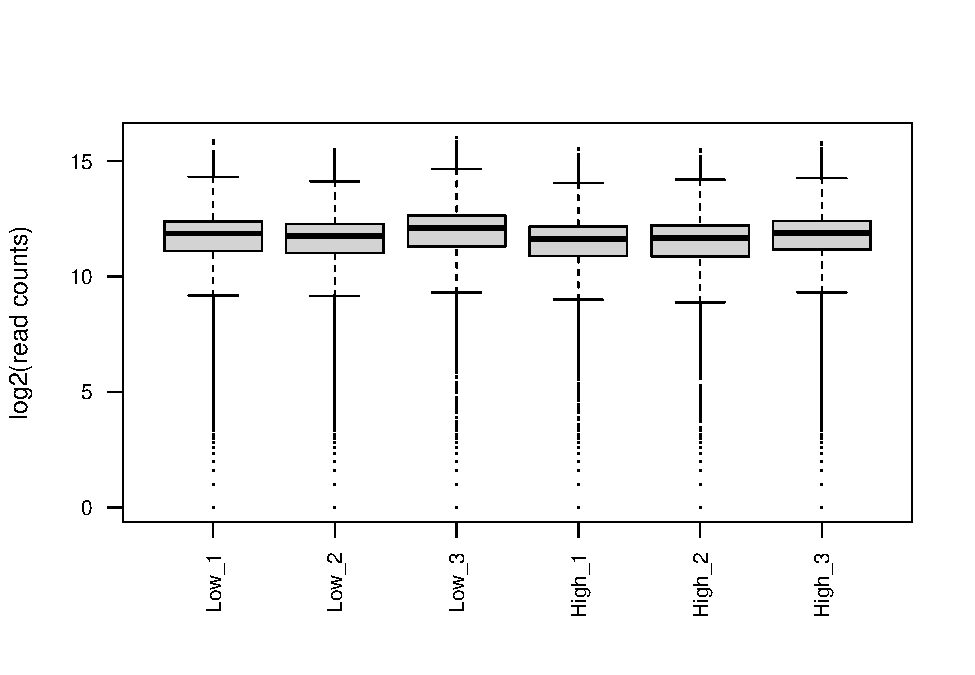
\includegraphics{all_countsummary-005}

The following figure shows the histogram of median-normalized read counts in all samples.


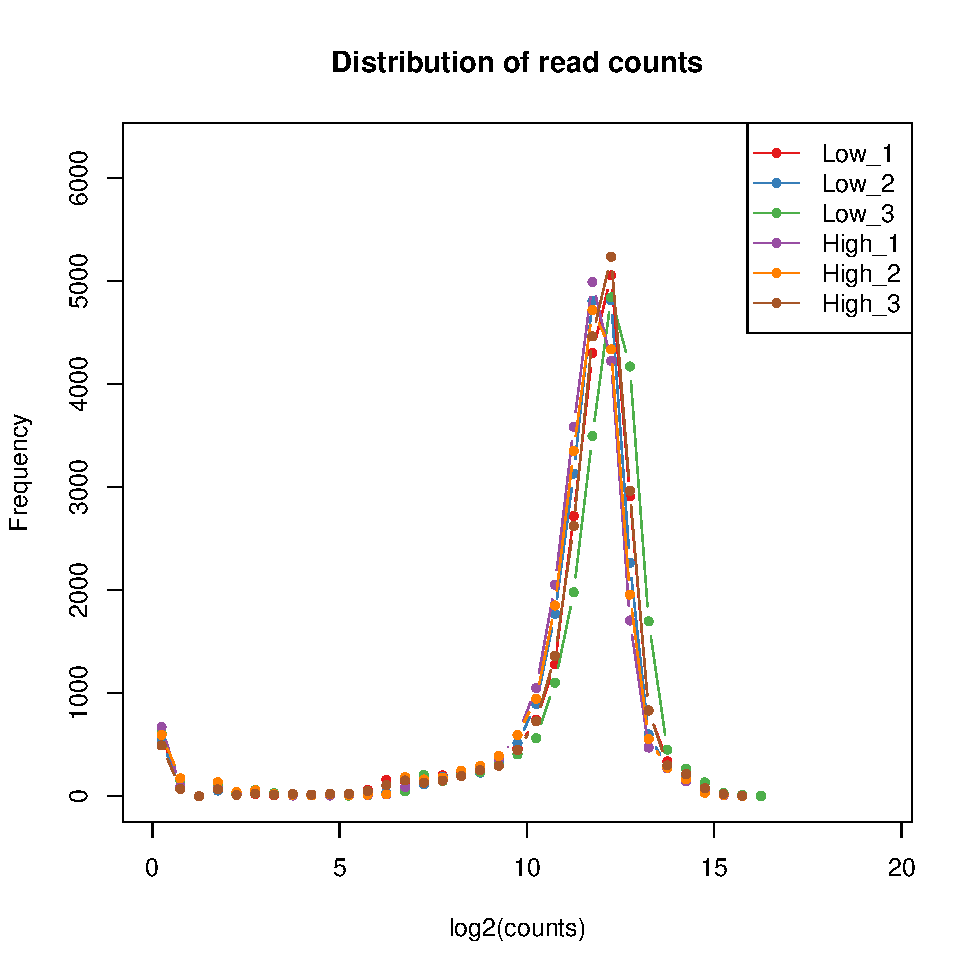
\includegraphics{all_countsummary-006}


\newpage\section{Principle Component Analysis}
The following figure shows the first 2 principle components (PCs) from the Principle Component Analysis (PCA), and the percentage of variances explained by the top PCs.



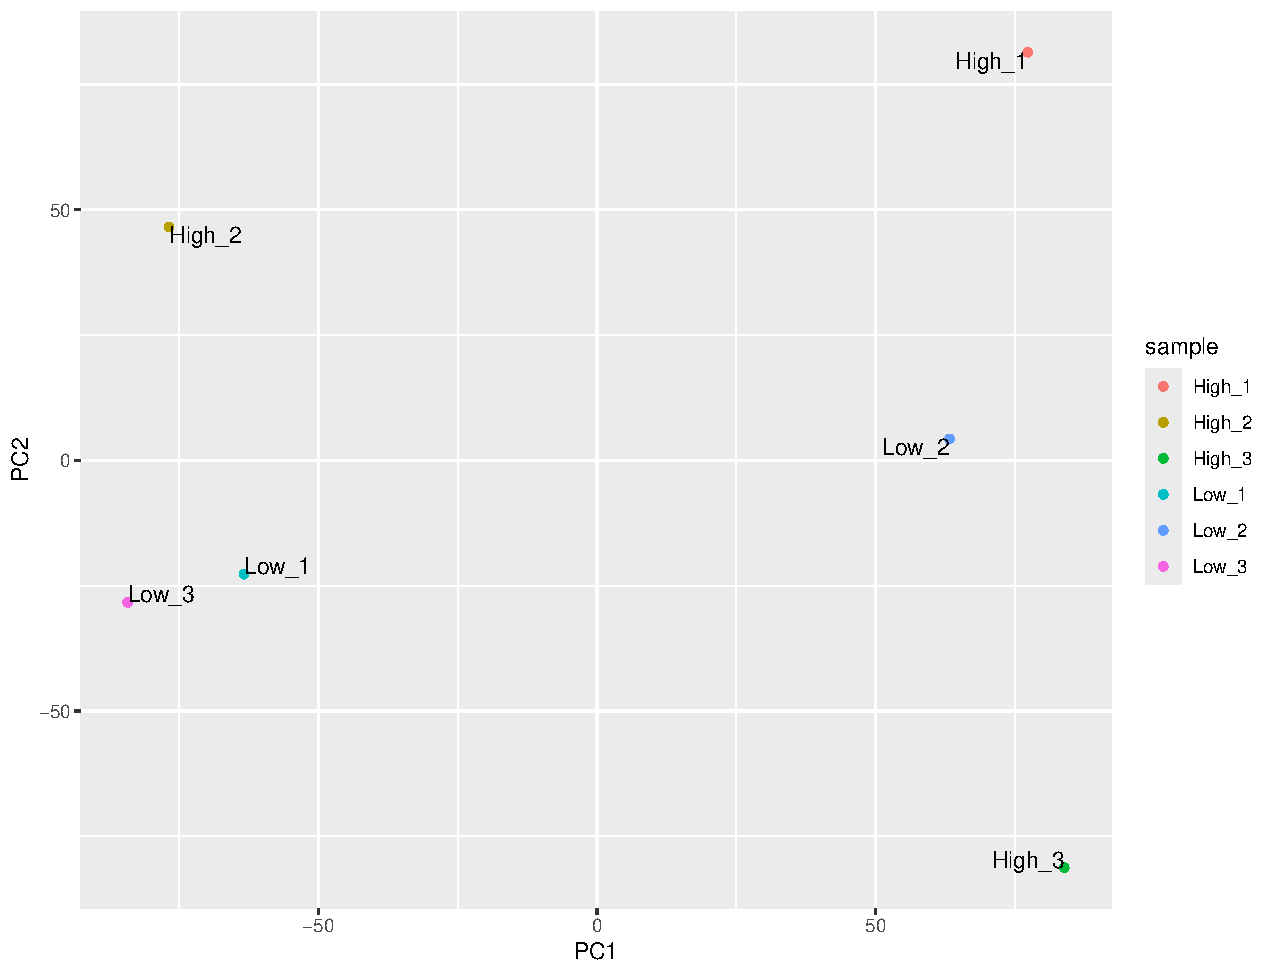
\includegraphics{all_countsummary-007}

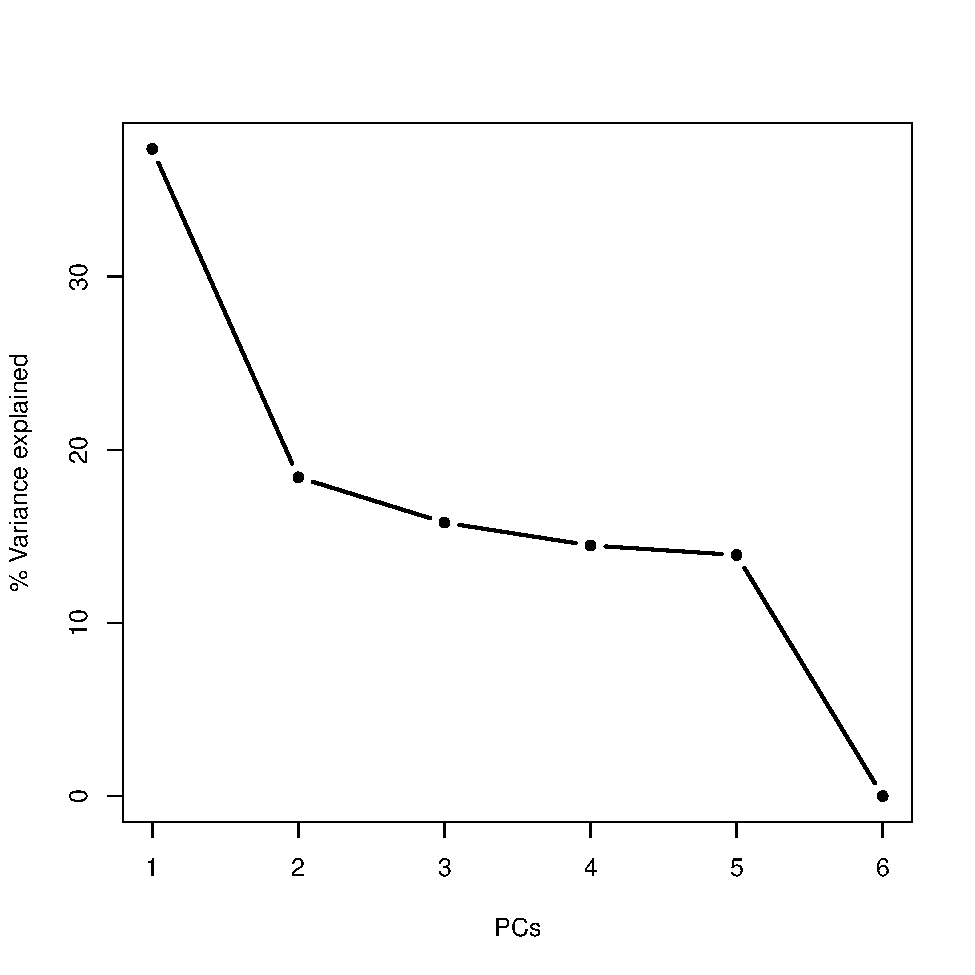
\includegraphics{all_countsummary-008}


\newpage\section{Sample clustering}
The following figure shows the sample clustering result.


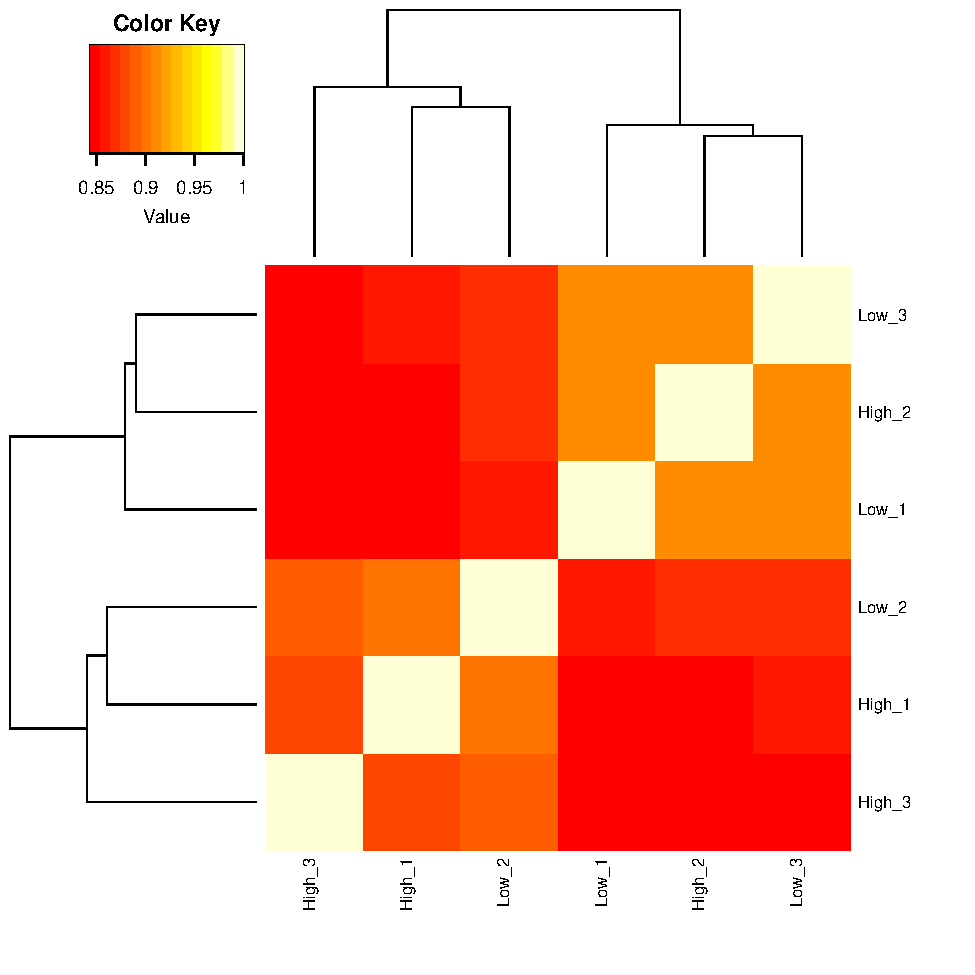
\includegraphics{all_countsummary-009}

%__INDIVIDUAL_PAGE__





\end{document}

